\documentclass{article}
\usepackage{graphicx} % Required for inserting images
\usepackage{amsmath} % For aligning equations
\usepackage{pgfplots} % For plotting graphs
\pgfplotsset{compat=1.18} % For pgfplots version 1.18 or later

\begin{document}
% Do not forget to \usepackage{graphicx} in the main
\begin{titlepage}

    % Students preferences
    \title{Physics Homework 2}
    \author{Ivan Chabanov\\i.chananov@innopolis.university\\DSAI-03}

    % Image
    \begin{figure}[t]
        \centering
        
\includegraphics[width=0.69\textwidth]{innou-logo.png} % Adjust accordingly if renamed
    \end{figure}

    % Title itself
    \maketitle

\end{titlepage}
 % Include the title page


% Solution #1
\section*{Problem 1 Statement}
The figure shows the time dependence of velocity. Do the following:

\begin{enumerate}
    \item Plot the acceleration and displacement with respect to time. Assume the initial coordinate is $x(0) = 0$ m.
    \item Determine the displacement and the average velocity over the time interval $[t_1, t_3]$.
\end{enumerate}

Given: $t_1 = 4$ s, $t_2 = 10$ s, $t_3 = 18$ s.

\section*{Solution}

\subsection*{1. Acceleration and Displacement Plots}

\subsubsection*{Acceleration}
Acceleration is the change of the velocity over the time interval.
We have 3 time intervals: 
\[
t_0 = 0s, \quad t_1 = 4s, \quad t_2 = 10s, \quad t_3 = 18s.
\]
Velocity in these intervals:
\[
v_0 = 0 m/s, \quad v_1 = 4m/s, \quad v_2 = 4m/s, \quad v_3 = 0m/s.
\]
Knowing these variables, we can find the acceleration:

$$ a_1 = \frac{v_1 - v_0}{t_1 - t_0} = \frac{4 - 0}{4 - 0}m/s^2 = 1m/s^2  $$
$$ a_2 = \frac{v_2 - v_1}{t_2 - t_1} = \frac{4 - 4}{10 - 4}m/s^2  = 0m/s^2  $$ 
$$ a_3 = \frac{v_3 - v_2}{t_3 - t_2} = \frac{0 - 4}{18 - 10}m/s^2  = -0.5m/s^2  $$
So the acceleration is $a(t) = \begin{cases} 1 & 0 \leq t \leq 4 \\ 0 & 4 < t \leq 10 \\ -0.5 & 10 < t \leq 18 \end{cases}$.

\subsubsection*{Displacement}
We know, that the displacement is the change of the coordinate over the time interval. Coordinate formula:

$$ x(t) = x(0) + v(0)t + \frac{1}{2}a(t) t^2 $$
As the point goes straight-line motion, the displacement could be found using the formula above.
Let us define a displacement over a time interval a:b as $ S_{[a:b]} $

$$ S_{[0:4]} = $$

\newpage %?

\textit{Acceleration figure:}

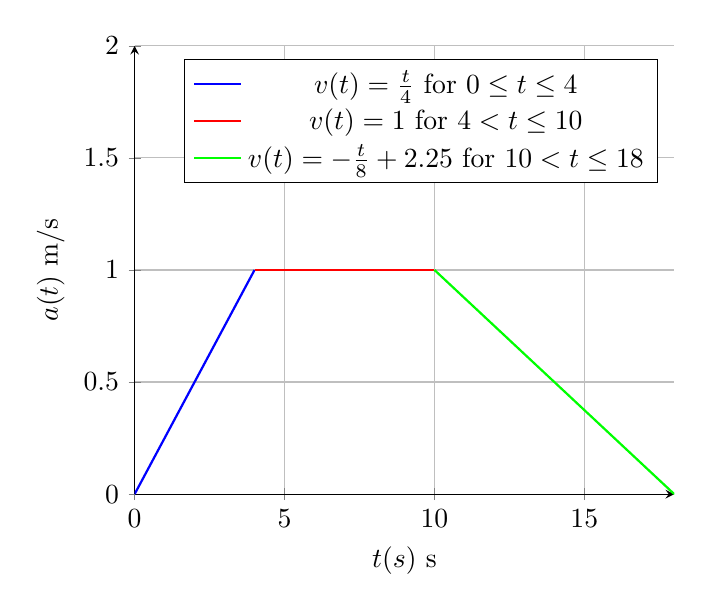
\begin{tikzpicture}
    \begin{axis}[
        axis lines = left,
        xlabel = $t(s)$ s,
        ylabel = {$a(t)$ m/s},
        ymin=0, ymax=2,
        xmin=0, xmax=18,
        legend pos=north east,
        samples=100,
        grid=major,
    ]

    % Plot for the first interval: v(t) = t/4 for 0 <= t <= 4
    \addplot[
        domain=0:4, 
        thick, 
        blue
    ] {x/4};
    \addlegendentry{$v(t) = \frac{t}{4}$ for $0 \leq t \leq 4$}

    % Plot for the second interval: v(t) = 1 for 4 < t <= 10
    \addplot[
        domain=4:10, 
        thick, 
        red
    ] {1};
    \addlegendentry{$v(t) = 1$ for $4 < t \leq 10$}

    % Plot for the third interval: v(t) = -x/8 + 2.25 for 10 < t <= 18
    \addplot[
        domain=10:18, 
        thick, 
        green
    ] {-x/8 + 2.25};
    \addlegendentry{$v(t) = -\frac{t}{8} + 2.25$ for $10 < t \leq 18$}

    \end{axis}
\end{tikzpicture}

\end{document}